\documentclass[12pt] {article}
\usepackage{times}
\usepackage[margin=1in,bottom=1in,top=0.6in]{geometry}

\usepackage{hhline}

\usepackage{float}
\usepackage{graphicx}
\usepackage{subfig}
\usepackage{wrapfig,lipsum}
\usepackage{amssymb}
\usepackage{nath}
\usepackage{amsfonts}
\usepackage{hyperref}
\begin{document}

\title{DLP Project Report}
\author{Ahmed H. Mahmoud}
\date{June, 8th 2017}
\maketitle

%============Part 1========
\section*{Part 1:}
For this part we are examining the effect of varying the number of registers on the performance. The experiments were done on \emph{Quadro 600} with Fermi architecture which allows up to 63 registers per thread. Varying the number of registers per thread has a direct impact on occupancy. Occupancy is an indication to the number of threads that run concurrently. Due to the fixed number of thread per SM, having fewer registers per threads will allow more threads (warps) to run concurrently and better latency hiding is achievable. This may come at the cost of spilling registers to local memory and the end results is lower performance. Thus, we need to experiment with varying number of registers that would lead to best performance. In all experiments, we don't allow register spilling. 

Figure \ref{fig:regs} shows the processing time for our kernel against different number of registers. In order to change the number of registers, we added more float (\emph{valXY}) computation. All the \emph{float valXY} have different values and thus adding new ones requires issuing more registers from the GPU side. The best performance is achieved with the least number of register used. Even though that this could be due to unbalanced workload between different experiments, but having fewer registers means that the SM can launch more warps that can run concurrently and higher throughout is attainable. 

\begin{figure}[!tbh]
 \centering        
   \subfloat {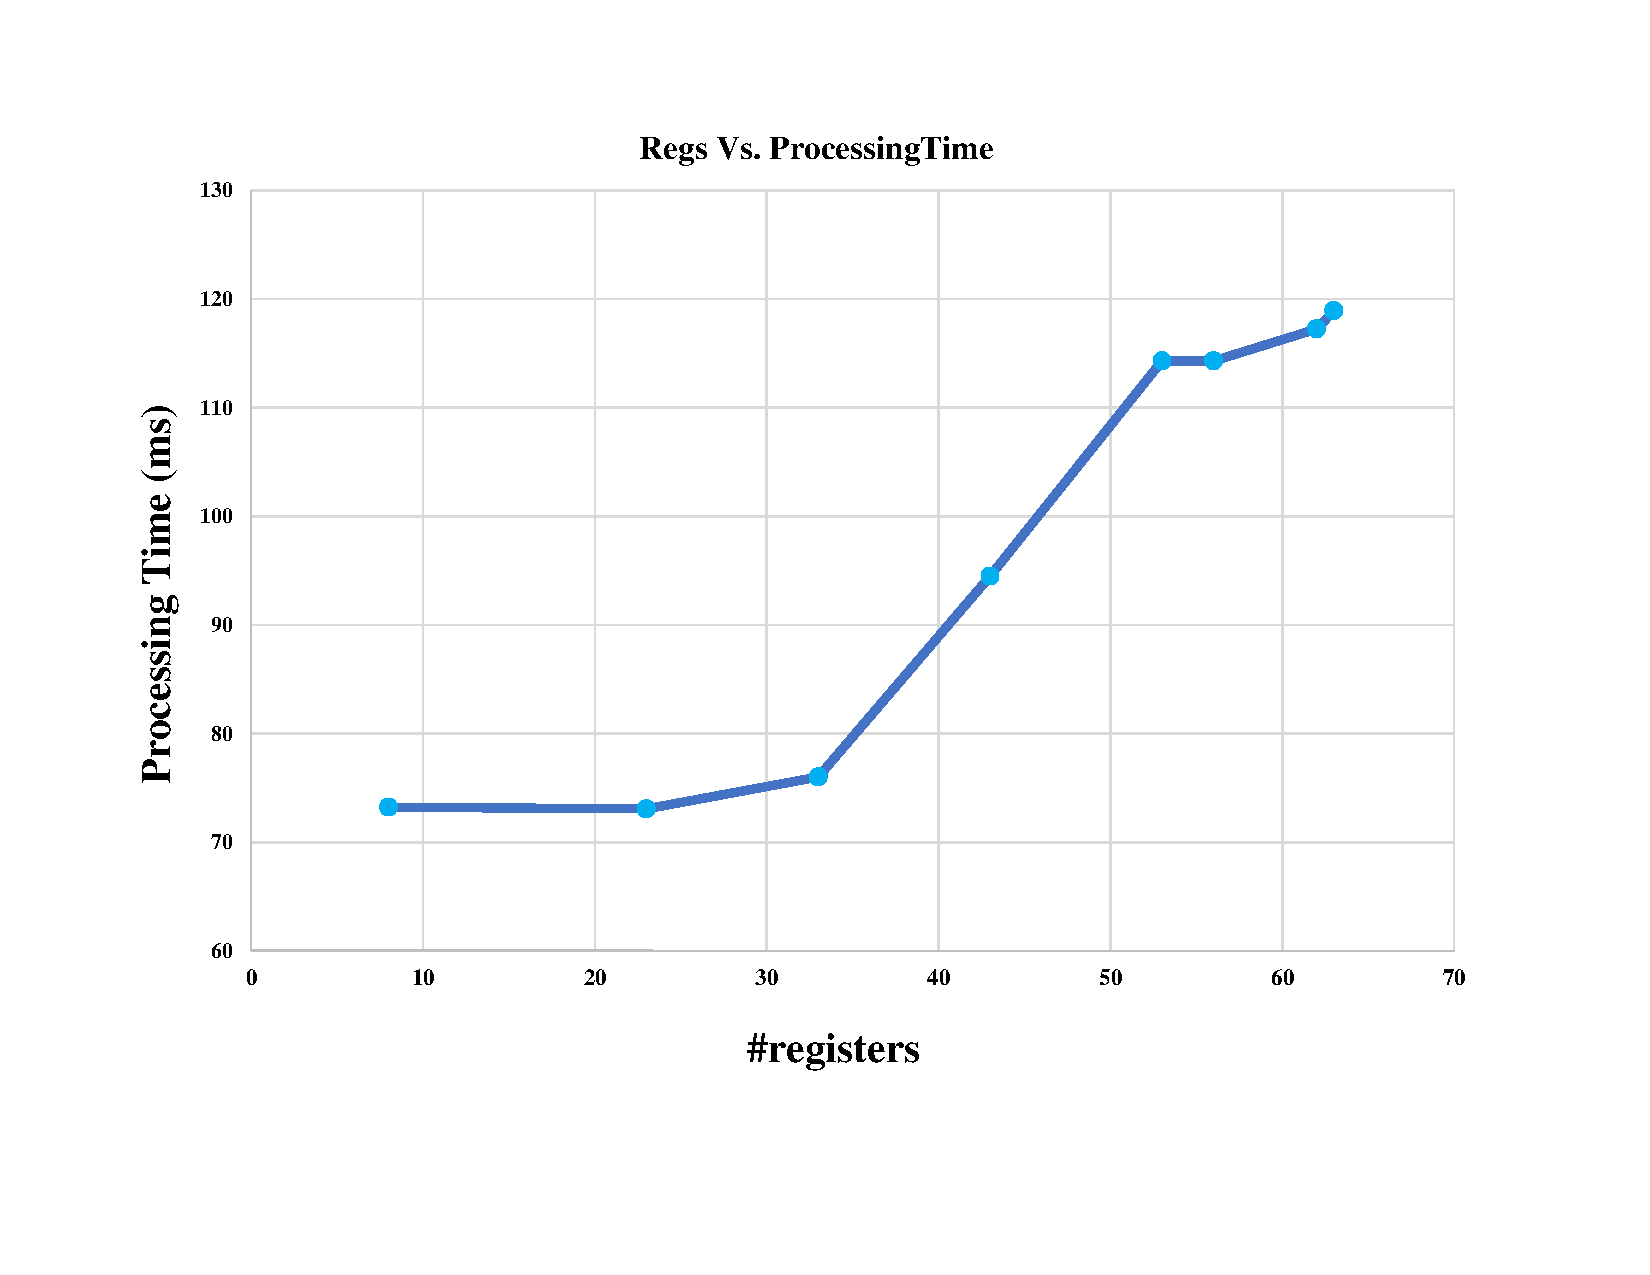
\includegraphics[width=0.7\textwidth]{regs/regs.pdf}}
     \caption{Number of registers Vs. processing time}
   \label{fig:regs}
\end{figure}  


%============Part 2========
\section*{Part 2:}
In this part we examine the parallelization of reduce operation across many threads and multiple blocks using only global memory. Reduce operation is done on one 1D float array of size $Nele=16384$ elements with sum operator. 

\paragraph{Method:}

The code run in two stages. In the first stage, we launch $\frac{Nele}{Nthreads}$ blocks, where $Nthreads$ is number of threads per block. Each block will reduce $Nthreads$ elements individually using the reduce kernel. In the second stage, we will run the same kernel to reduce number of elements equal to the number of blocks launched in the first stage to reduce the results stored in each block from stage one. 

The reduce kernel runs a loop over the active region (across threads as in the first stage or across blocks as in the second stage). In each iteration, we divide the active region in half where each half compute the sum of its values and the other half. The loop continue halving the active regions and synchronizing across all threads at the end of each iteration until there is only one element then the loop terminates. In each iteration, the read and write are done from the global memory which we will change in Part 3.  

\paragraph{Experiment:} Figure \ref{fig:reduce}(a) shows the performance of our reduce kernel using different number of threads. Using less number of threads means that a block would have to do multiple computation in each loop iterations which requires scheduling (serializing) the process. In contrast, when using many threads per block, all computation in one iteration can run in parallel which maximizes the throughput and hence better performance is achieved. We notice that when we used maximum number of threads per block ($1024$), the computation starts to slow down a little. We assume that this might be due to an overhead of launching too many threads such that it affects the run time negatively. 
\begin{figure}[!tbh]
 \centering        
   \subfloat [Global Memory] {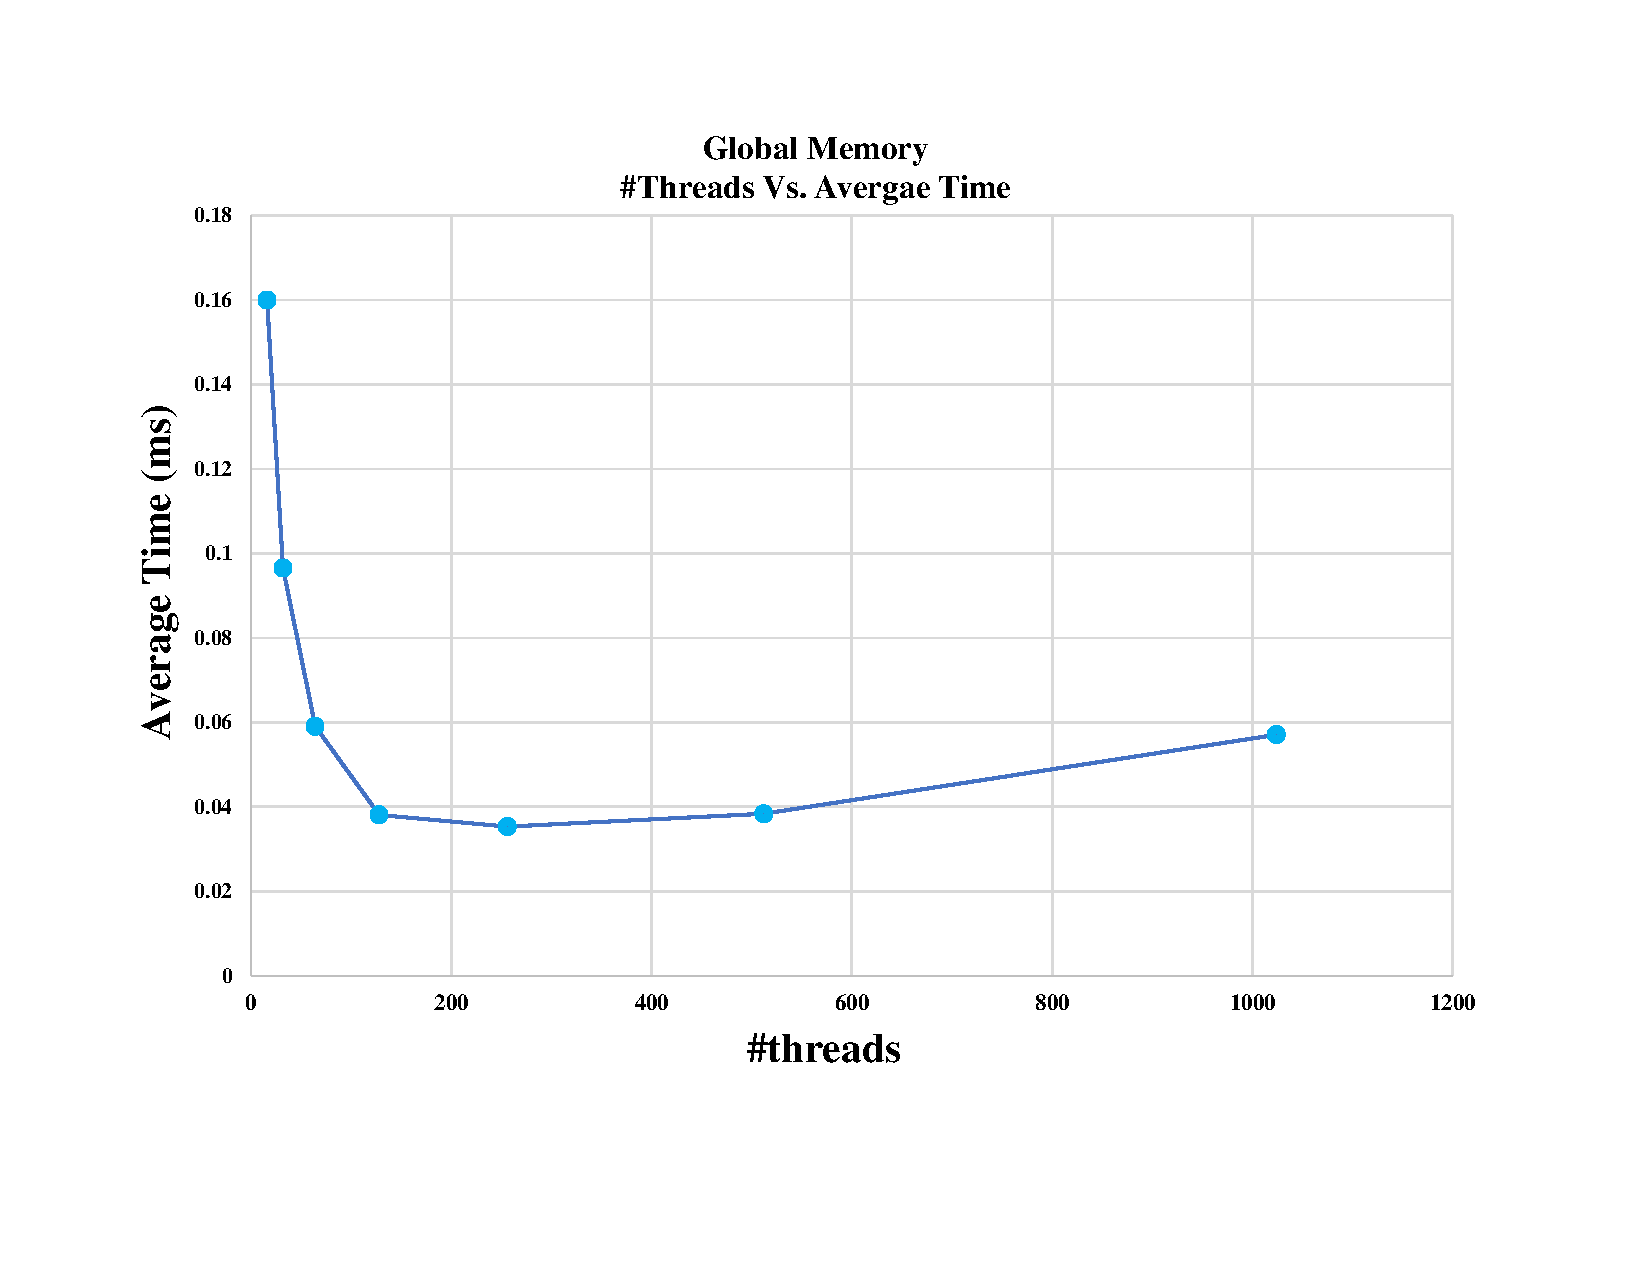
\includegraphics[width=0.48\textwidth]{reduce/global.pdf}}
   \subfloat [Shared Memory] {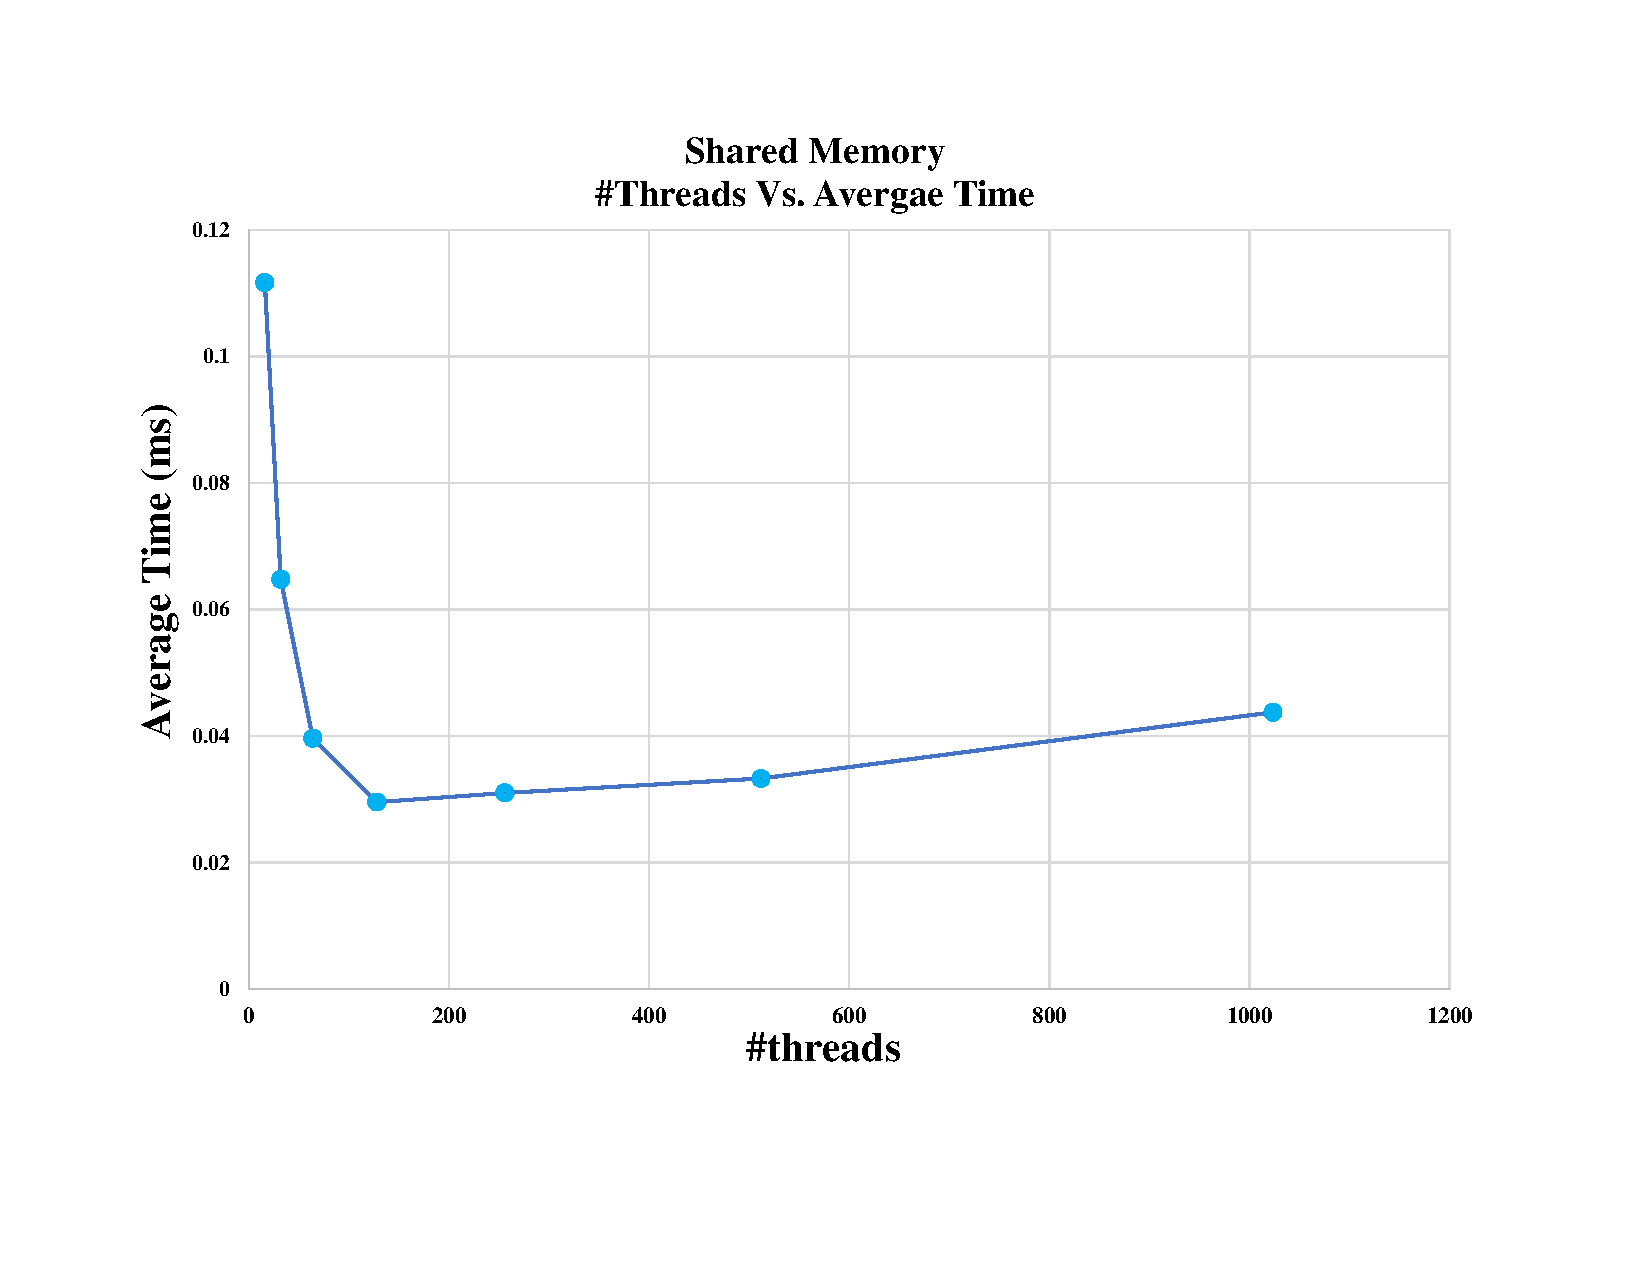
\includegraphics[width=0.48\textwidth]{reduce/shared.pdf}}
     \caption{Number of threads Vs. processing time for the reduce primitive.}
   \label{fig:reduce}
\end{figure}


%============Part 3========
\section*{Part 3:}
In this part, we used the shared memory for the intermediate write/read except for the first read when we read the input array into the shared memory and the final write where we write to the output array. Since the shared memory is closer to the threads within a block and has lower latency, using the shared memory for the intermediate write/read will have better performance. We experimented using different number of registers and reported the processing time as shown in Figure \ref{fig:reduce}(b). On average, the speedup obtained due to using shared memory is $23.8\%$. 


\section*{Notes on the code:}
In order to use the global memory, uncomment lines 204 and 209 and comment lines 205 and 2104. To use the shared memory, do the reverse. Using the global memory, the input array is being written inside the kernel by the intermediate values. Thus, when running many iterations in order to get the average processing time right, the test against the reference CPU computation fails. Using one iteration, the GPU code always passes the test. 

\end{document}


 